\documentclass[10pt]{beamer}

\usetheme[progressbar=frametitle]{metropolis}
\usepackage{appendixnumberbeamer}
\usepackage{subcaption}
\usepackage{booktabs}

\usepackage[scale=2]{ccicons}
\usepackage{svg}

\usepackage{pgfplots}
\usepgfplotslibrary{dateplot}
\usepackage{graphicx}
\usepackage{xspace}
\newcommand{\themename}{\textbf{\textsc{metropolis}}\xspace}
\usepackage{amsmath, amssymb, latexsym}
\usepackage{sidecap}
 \setbeamertemplate{caption}{\raggedright\insertcaption\par}

\usepackage{tikz}
\usetikzlibrary{decorations.pathreplacing}

\title{Persistent homology}
\subtitle{A gentle introduction}
% \date{\today}
\date{}
\author{Daniel Collin}
\setbeamercolor{background canvas}{bg=white}

% \institute{Center for modern beamer themes}
% \titlegraphic{\hfill\includegraphics[height=1.5cm]{logo.pdf}}
\begin{document}
% \begin{frame}[fragile]{}
% \begin{figure}[ht]
%   \centering
%   \begin{subfigure}[t]{.5\linewidth}
%     \caption{\label{annulus:points}}
%  \end{subfigure}%
%   \begin{subfigure}[t]{.5\linewidth}
%     \caption{\label{annulus:imposed}}
%  \end{subfigure}
% \end{figure}
% \end{frame}

\begin{frame}[fragile]{Two questions}
  \begin{enumerate}
          \item Correlation between ITW and topology of the eye?
          \item Can we group BT samples based on PH that correspond with size?
          \end{enumerate}
          \begin{itemize}
            \item Persistent homology is a good choice, measures shape not size.
                  \item $H_{1}$ encodes loops in volume, $H_{2}$ encodes voids in volume.
                  \end{itemize}
\end{frame}
\begin{frame}[fragile]{Setup}

  \begin{itemize}
    \item<1-> Two groups, one consisting of \textit{Bombus terrestris} and one of others
    \item<2-> We compute \textit{persistent homology} for the cornea of each sample (less noisy)
    \item<3-> We create a distance matrix that tells us how close each sample is to the other (topologically, ITW)
    \item<4-> Mantel test each group separately with PH matrix and ITW matrix
    \item<5-> Cluster \textit{Bombus terrestris} based on best metric from Mantel test
  \end{itemize}


\end{frame}
\begin{frame}[fragile]{Mantel test results}
\begin{table}[ht]
  \centering
\begin{tabular}{*6l}    \toprule
Group  & Metric  & $H_{1} \rho $  & $H_{1}$ p-value  & $H_{2} \rho$ & $H_{2}$ p-value  \\ \midrule
\textit{BT} & Bottleneck & $-0.069$ & $0.84$ & $0.86$ & $0.0083$\\
\textit{BT} & Wasserstein & $0.59 $ & $0.053 $ & $0.49$ & $0.080$\\
\textit{Others}& Bottleneck & $0.22$ & $0.030$ & $0.33$ & $0.0073$\\
\textit{Others}& Wasserstein & $0.23$ & $0.023$ & $0.26$ & $0.013$\\\bottomrule
 \hline
\end{tabular}
\end{table}
$H_{2}$ with bottleneck distance shows significant results for \textit{Bombus terrestris} and the other group of insects.
\end{frame}

\begin{frame}[fragile]{Clustering on $H_{2}$ (bottleneck)}

  \begin{figure}
    \begin{tabular}{3l}
    ID & ITW \\
    \midrule
    BT\_77976 & 5.47 \\
    BT\_77967 & 5.42 \\
    BT\_77971 & 4.02 \\
    BT\_77970 & 4.00 \\
    BT\_77974 & 2.97 \\
    BT\_77973 & 1.97
      \end{tabular}
    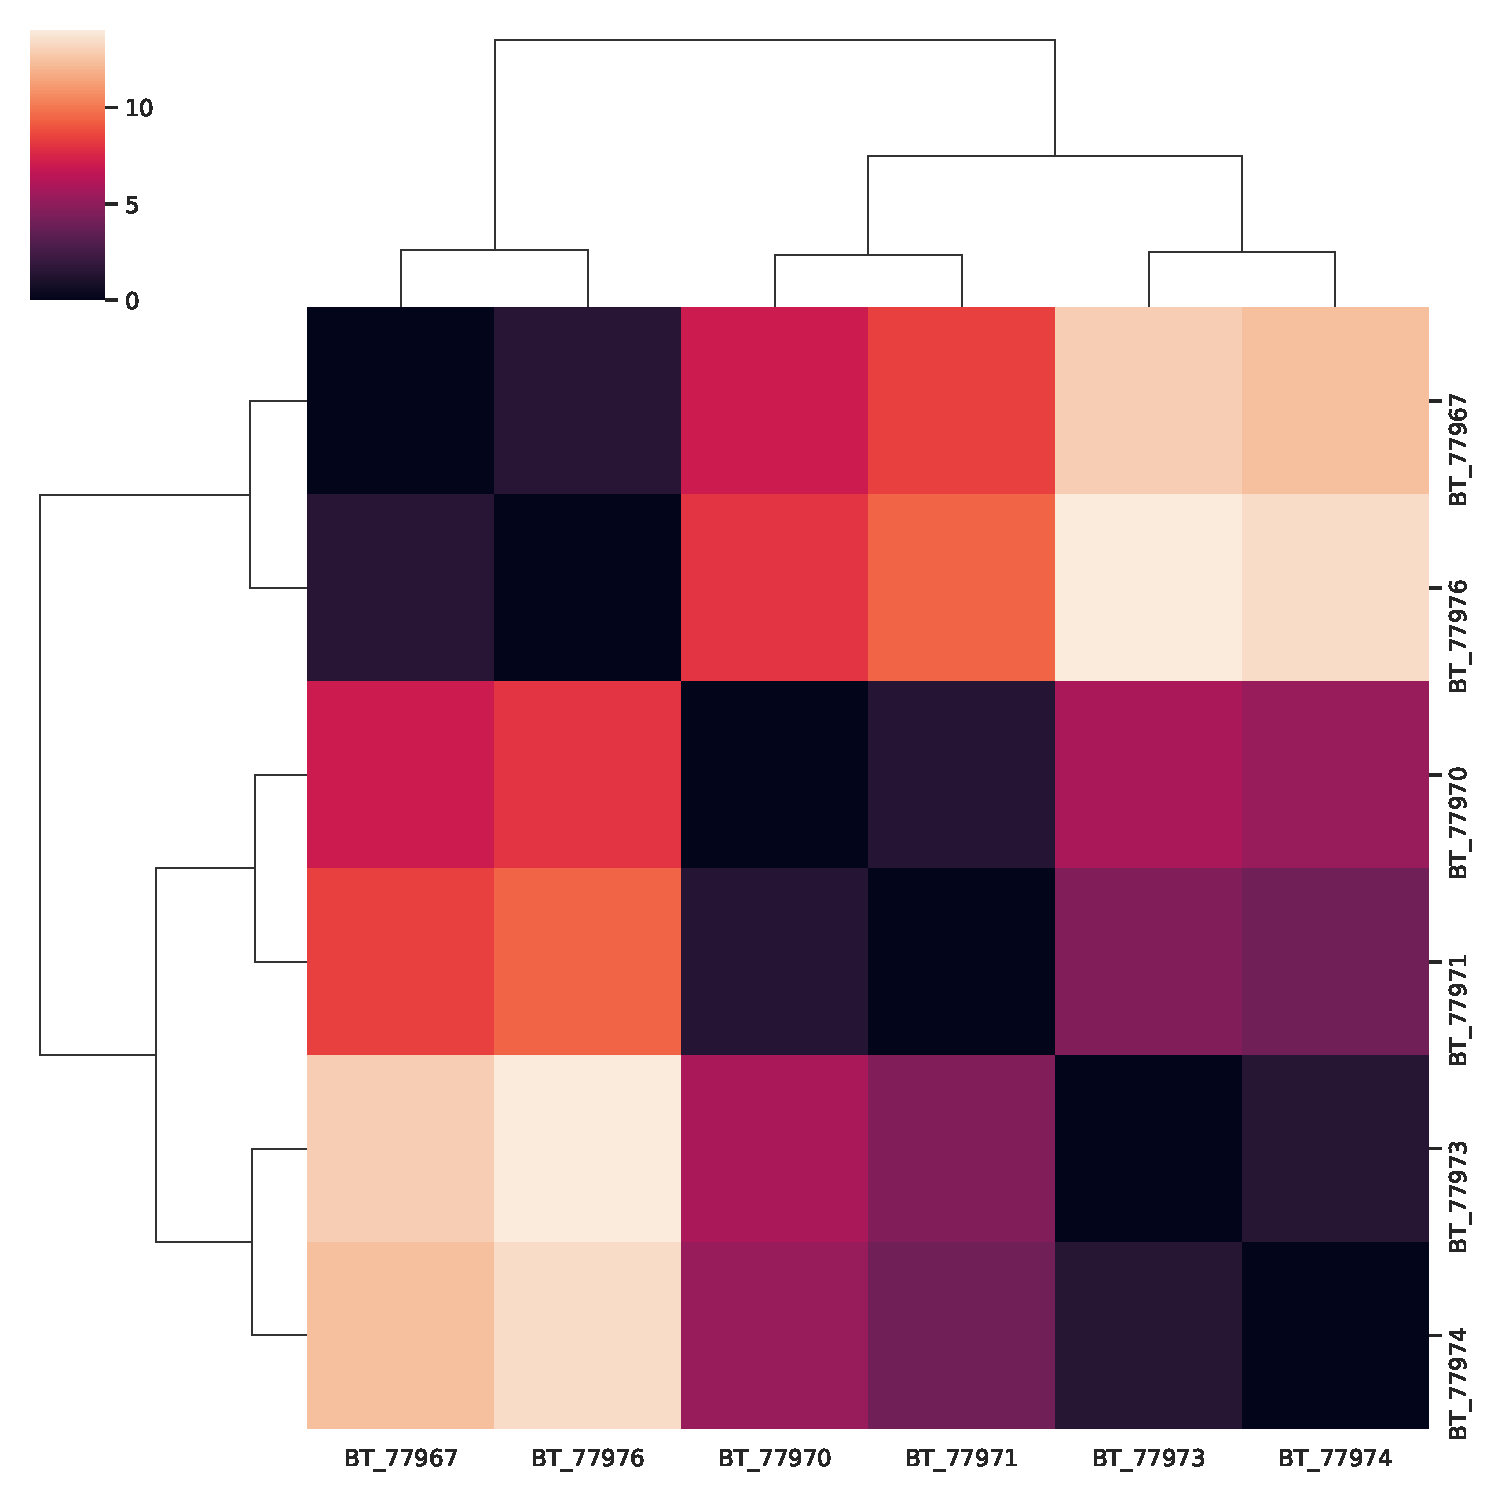
\includegraphics[scale=0.25]{./clusters/bottleneck_h2_cluster.pdf}
  \end{figure}
  \end{frame}
\begin{frame}[fragile]{Conclusions}
  \begin{itemize}
    \item Supports the hypothesis that ITW and topology of eye are related
    \item Other dimensions/metrics were not as correlated, but do we want strong correlation?
  \end{itemize}
  \end{frame}
\end{document}
